\section{Auswertung}

\subsection{Emissionsspektrum der Kupfer-Röntgenröhre}

Das Emissionsspektrum der Kupfer-Röntgenröhre wurde mit einer Integrationszeit von $\increment t = \SI{10}{\second}$ in jeweils $\increment \theta = 0{,}1\textdegree$ Abständen gemessen.
Diese Zählraten am Geiger-Müllerzählrohr lassen sich nun im Diagramm \ref{fig:plot1} in Abhängigkeit vom Winkel $\theta$ darstellen.
Der Bremsberg ist im Diagramm durch schwarze Punkte dargestellt, sie zeigen die Strahlung welche durch Abbremsung der Elektronen am Kupfer entsteht. 
Außerdem sind zwei charakteristische Linien zu erkennen, die $K_{\beta}$ und $K_{\alpha}$-Linie.

\begin{figure}[h]
  \centering
  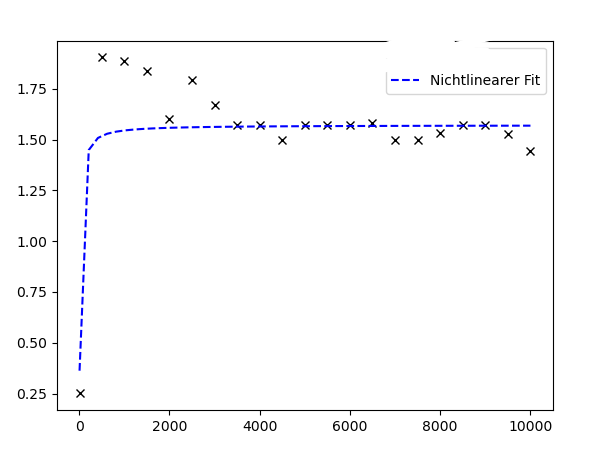
\includegraphics[width=\textwidth]{build/plot1.pdf}
  \caption{Röntgenspektrum einer Kupfer-Röntgenröhre.}
  \label{fig:plot1}
\end{figure}

Diese Linien lassen sich am Diagramm \ref{fig:plot1} und den gemessenen Werten in Tabelle \ref{tab:cuwerte1} grob ablesen zu.

\begin{align*}
K_{\alpha} &= 22{,}5\textdegree \\
K_{\beta} &= 20{,}2\textdegree
\end{align*}
Aus diesen Winkeln lässt sich mit der aufgestellten Beziehung \eqref{eqn:braggEnergy} die Energie dieser K-Linien berechnen. Hierbei wird die Beugungsordnung $n = 1$ betrachtet.
Es ergeben sich die Werte.
\begin{align}
E_{\text{K,}\alpha} &= \SI{8.043}{\kilo\electronvolt} \\
E_{\text{K,}\beta} &= \SI{8.914}{\kilo\electronvolt}
\end{align}
Die Abweichungen zu den angegebenen Literaturwerten \ref{tab:vorbereitung} sind in der folgenden Tabelle \ref{tab:litabweichung1} in Prozent angegeben.
\begin{table}
\centering
\caption{Prozentuale Abweichung zu den Literaturwerten.}
\label{tab:litabweichung1}
\begin{tabular}{c c c}
    \toprule
    Linie & Energieabweichung & Winkelabweichung \\
    \midrule
    $K_{\alpha}$     &  $\SI{0.058}{\percent}$ &  $\SI{0.044}{\percent}$    \\
     $K_{\beta}$     &  $\SI{0.081}{\percent}$ &  $\SI{0.099}{\percent}$   \\
    \bottomrule
\end{tabular}
\end{table}